\documentclass[border=10pt]{standalone}
\usepackage{tikz}
\usetikzlibrary{positioning, arrows.meta, calc}

\definecolor{coloredge}{HTML}{222222} % Darker, crisper edge color for unshaded boxes

\begin{document}
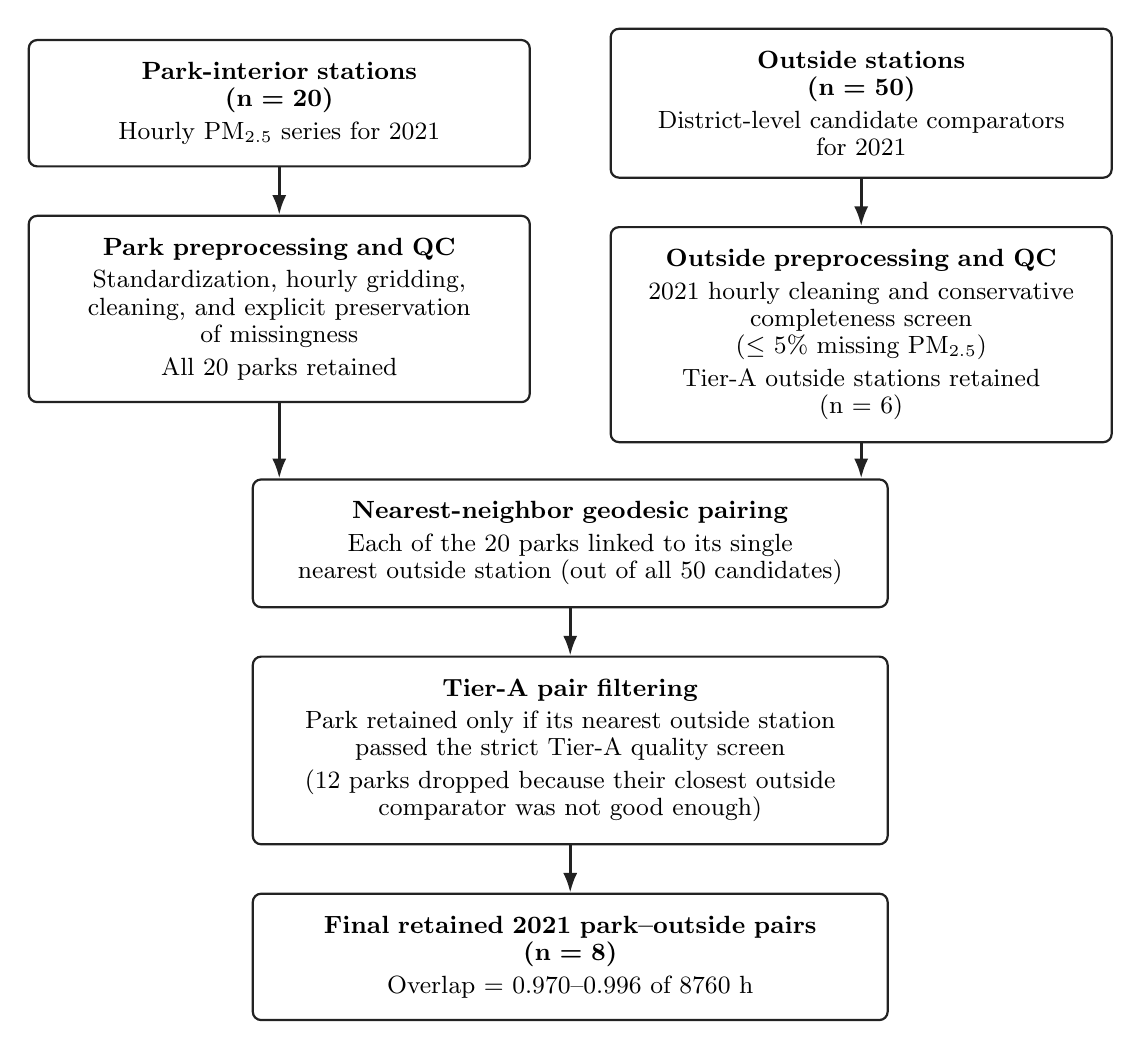
\begin{tikzpicture}[
    % Tighter vertical spacing between boxes
    node distance=0.6cm and 1cm,
    % Define the clean, unshaded style for all boxes
    box/.style={
        rectangle,
        draw=coloredge,
        fill=white, % Removed all background colors
        rounded corners=3pt, % Slightly sharper, modern corners
        align=center,
        text width=5.8cm,
        minimum height=1.2cm,
        inner sep=8pt,
        line width=0.8pt,
        text=black,
        font=\linespread{0.9}\small % Removed \sffamily to use the default serif font
    },
    % Style for the wider center boxes at the bottom
    widebox/.style={
        box,
        text width=7.5cm
    },
    % Sleek, modern arrow style
    arrow/.style={
        -{Latex[length=2.5mm, width=1.8mm]},
        coloredge,
        line width=1.0pt
    }
]

% ==============================
% Row 1: Inputs
% ==============================
\node[box] (park) {
    \textbf{Park-interior stations} \\
    \textbf{(n = 20)} \\[0.2em]
    Hourly PM$_{2.5}$ series for 2021
};

\node[box, right=of park] (outside) {
    \textbf{Outside stations} \\
    \textbf{(n = 50)} \\[0.2em]
    District-level candidate comparators \\
    for 2021
};

% ==============================
% Row 2: QC
% ==============================
\node[box, below=of park] (parkqc) {
    \textbf{Park preprocessing and QC} \\[0.2em]
    Standardization, hourly gridding, \\
    cleaning, and explicit preservation \\
    of missingness \\[0.2em]
    All 20 parks retained
};

\node[box, below=of outside] (outsideqc) {
    \textbf{Outside preprocessing and QC} \\[0.2em]
    2021 hourly cleaning and conservative \\
    completeness screen ($\leq$ 5\% missing PM$_{2.5}$) \\[0.2em]
    Tier-A outside stations retained \\
    (n = 6)
};

% ==============================
% Row 3: Pairing
% ==============================
\node[widebox, below=0.7cm of $(parkqc.south)!0.5!(outsideqc.south)$] (pairing) {
    \textbf{Nearest-neighbor geodesic pairing} \\[0.2em]
    Each of the 20 parks linked to its single \\
    nearest outside station (out of all 50 candidates)
};

% ==============================
% Row 4: Filtering
% ==============================
\node[widebox, below=0.6cm of pairing] (filter) {
    \textbf{Tier-A pair filtering} \\[0.2em]
    Park retained only if its nearest outside station \\
    passed the strict Tier-A quality screen \\[0.2em]
    (12 parks dropped because their closest outside \\
    comparator was not good enough)
};

% ==============================
% Row 5: Final
% ==============================
\node[widebox, below=0.6cm of filter] (final) {
    \textbf{Final retained 2021 park--outside pairs} \\
    \textbf{(n = 8)} \\[0.2em]
    Overlap = 0.970--0.996 of 8760 h
};

% ==============================
% Arrows
% ==============================
\draw[arrow] (park) -- (parkqc);
\draw[arrow] (outside) -- (outsideqc);

% Draw perfectly vertical straight lines from the QC boxes down to the Pairing box
\draw[arrow] (parkqc.south) -- (parkqc.south |- pairing.north);
\draw[arrow] (outsideqc.south) -- (outsideqc.south |- pairing.north);

\draw[arrow] (pairing) -- (filter);
\draw[arrow] (filter) -- (final);

\end{tikzpicture}
\end{document}